We are now going to consider a more complex geometry. The L-shaped area and the corresponding "normal" mesh are given in figure \ref{Lmesh}.

\begin{figure}
\begin{center}
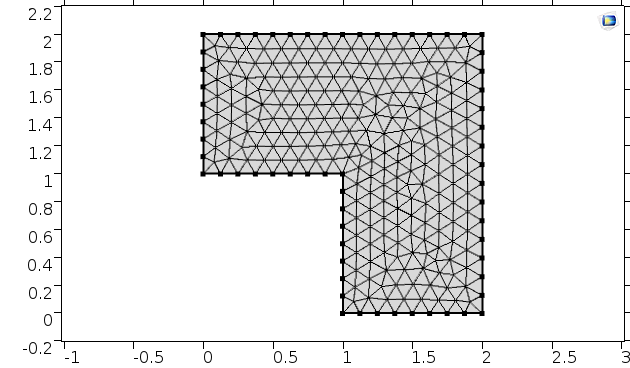
\includegraphics[scale=0.6]{Lmesh.png}
\caption{Geometry and mesh for the L-shaped domain}
\label{Lmesh}
\end{center} 
\end{figure}

This mesh contains 489 triangles and 1042 degrees of freedom. There are also 277 nodes. The solution computed by Comsol is given in figure \ref{laplaceL}. For this mesh, we have the following values :

\begin{align*}
T(1,1)&=450.0000144393805   \\
T(2,2)&=449.9890727451373
\end{align*}

\begin{figure}
\begin{center}
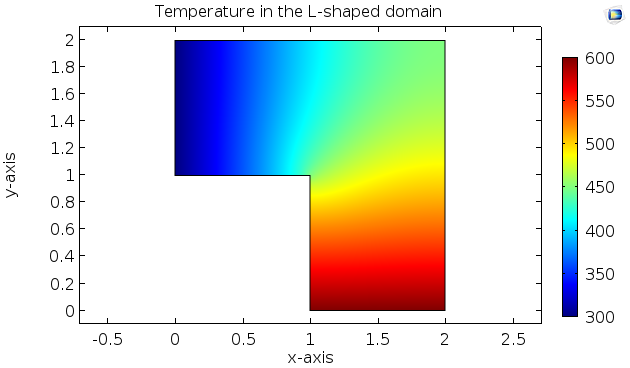
\includegraphics[scale=0.6]{laplaceL.png}
\caption{Solution for the L-shaped domain}
\label{laplaceL}
\end{center}
\end{figure}


We are now going to refine the mesh again. The mesh "fine" will be chosen. It contains 739 triangles and 1558 degrees of freedom. There are also 410 nodes. With this mesh, we find : 

\begin{align*}
T(1,1)&=450.00002426286386   \\
T(2,2)&=449.9903296071951
\end{align*}

It is easy to see that for the two meshes, $T(1,1)$ and $T(2,2)$ are very close to $450$.

Finally, we are going to refine the regions around $(1,1)$ and $(2,2)$. For $(1,1)$, we use a corner refinement and for $(2,2)$ we use a box refinement. Figure \ref{refine} shows the refined mesh. This new mesh contains 708 triangles and 1493 degrees of freedom, as well as 393 nodes.

\begin{figure}
\begin{center}
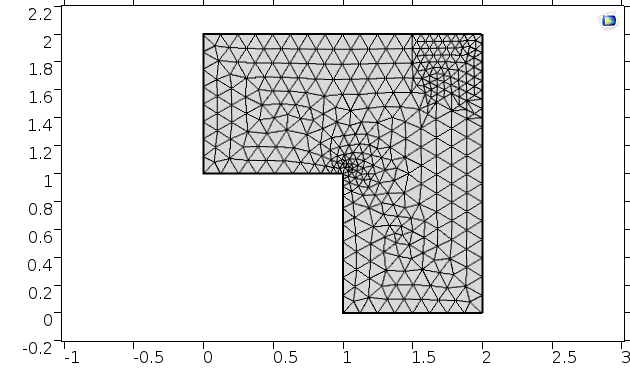
\includegraphics[scale=0.6]{refine.png}
\caption{Refined mesh}
\label{refine}
\end{center}
\end{figure}

The values of $T$ are :
\begin{align*}
T(1,1)&=449.99995663599896   \\
T(2,2)&=449.9952016386103
\end{align*}

Once again, we can see that the values are really close to 450.